\begin{figure}[htbp]
\centering
\begin{tikzpicture}[x=1cm,y=1cm]
\node[anchor=south west,inner sep=0] at (0,0) {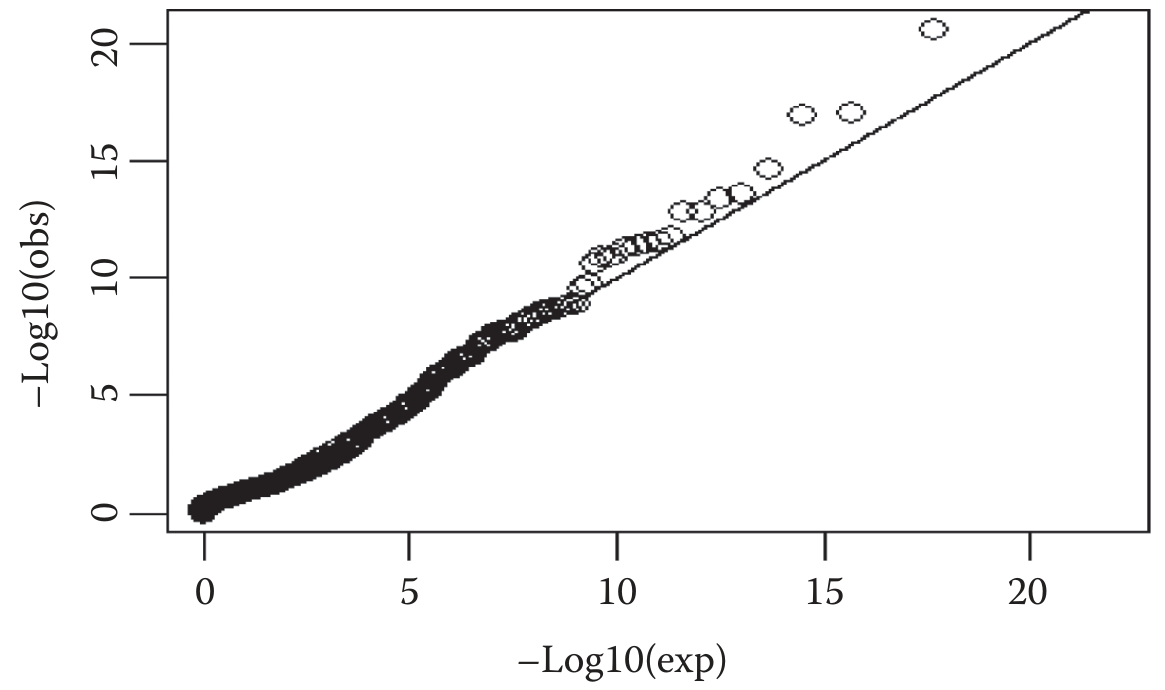
\includegraphics[width=13.0cm]{figures/ch03_fig19_data.png}};
\fill[white] (5.7310,0.0659) rectangle (8.1567,0.5681);
\node[font=\small,rotate=0,inner sep=0] at (6.9439,0.3170) {$-\log_{10}(\text{期望值})$};
\fill[white] (0.1613,3.1085) rectangle (0.6746,5.5141);
\node[font=\small,rotate=90,inner sep=0] at (0.4180,4.3113) {$-\log_{10}(\text{观测值})$};
\end{tikzpicture}
\origfig{19}{QQ 图。}
\label{fig:ch03-19}
\end{figure}
